\documentclass[tikz,border=10pt]{standalone}
\usepackage{helvet}
\renewcommand{\familydefault}{\sfdefault}
\usepackage{tikz}
\usetikzlibrary{arrows.meta, positioning, calc, shapes.geometric, decorations.pathreplacing}

\definecolor{emeraldpine}{HTML}{1A4D3E}
\definecolor{harvardcrimson}{HTML}{A51C30}
\definecolor{ethdarkblue}{HTML}{1F407A}
\definecolor{ethpetrol}{HTML}{007A87}
\definecolor{ethbronze}{HTML}{B87333}
\definecolor{ethpurple}{HTML}{5B4B8A}
\definecolor{ink}{HTML}{1A202C}
\definecolor{softink}{HTML}{4A5568}
\definecolor{paleink}{HTML}{A0AEC0}
\definecolor{cardbg}{HTML}{F8FAFC}
\definecolor{shadecolor}{HTML}{F4F6F9}

\begin{document}
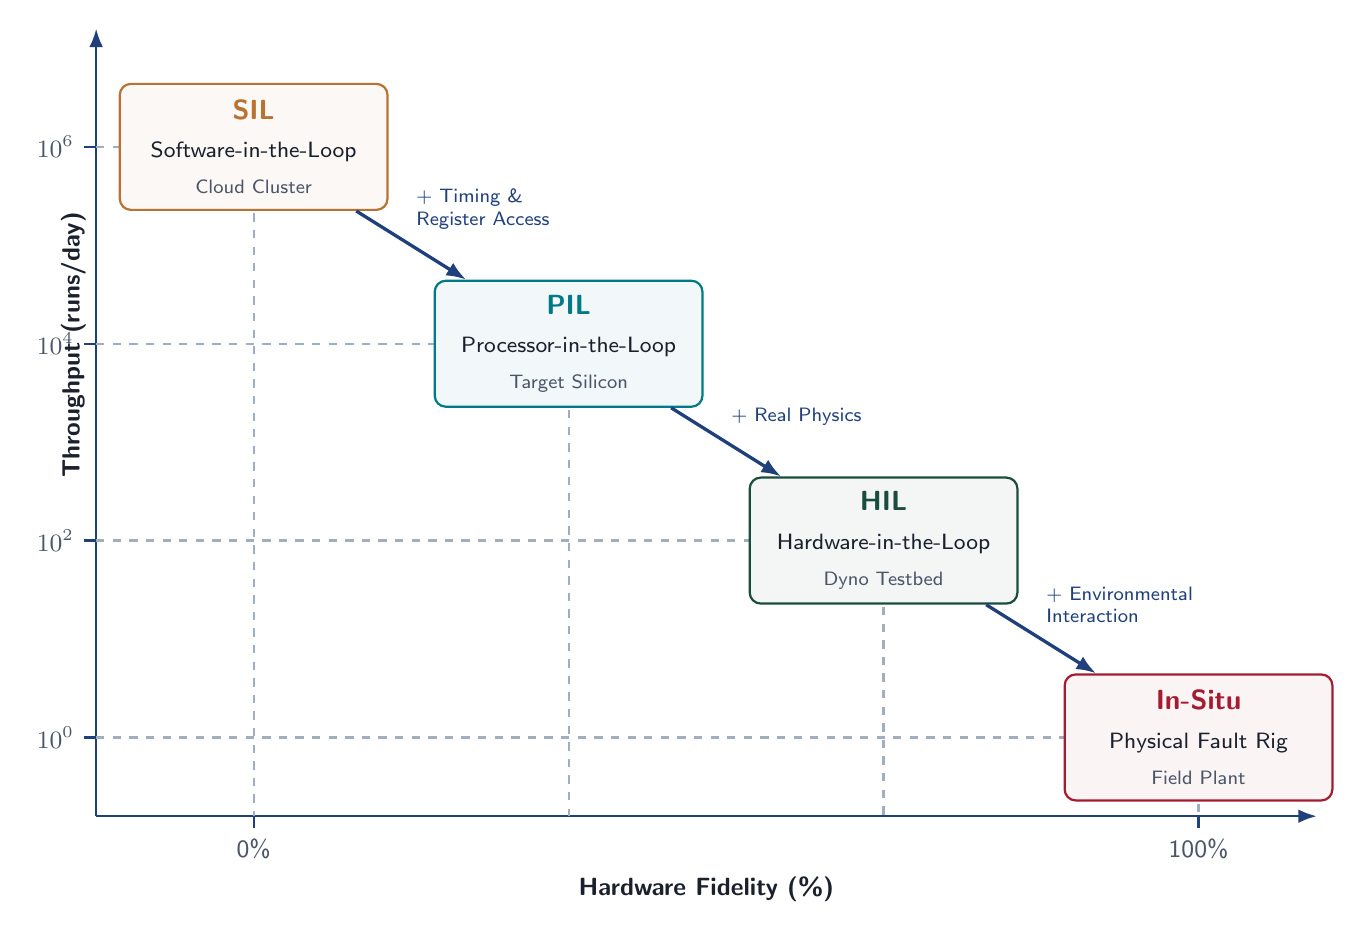
\begin{tikzpicture}[
    >=Latex,
    font=\sffamily,
    stagebox/.style={
        rectangle, 
        rounded corners=4pt,
        draw=#1, 
        thick, 
        fill=#1!5, 
        minimum width=3.4cm, 
        minimum height=1.6cm, 
        align=center,
        text=ink
    },
    axis/.style={->, thick, ethdarkblue},
    tick/.style={ethdarkblue, thick},
    proj/.style={dashed, paleink, thick},
    arrow/.style={->, thick, ethdarkblue}
]

% Coordinates
% X-axis: 0 to 15.5
% Y-axis: 0 to 10

% Axes
\draw[axis] (0,0) -- (15.5,0) node[midway, below=18pt, font=\bfseries\small, text=ink] {Hardware Fidelity (\%)};
\draw[axis] (0,0) -- (0,10) node[midway, above=28pt, rotate=90, font=\bfseries\small, text=ink] {Throughput (runs/day)};

% Ticks X
\draw[tick] (2,0) -- (2,-0.15) node[below, text=softink, font=\small] {0\%};
\draw[tick] (14,0) -- (14,-0.15) node[below, text=softink, font=\small] {100\%};

% Ticks Y
\draw[tick] (0,1) -- (-0.15,1) node[left, text=softink, font=\small] {$10^0$};
\draw[tick] (0,3.5) -- (-0.15,3.5) node[left, text=softink, font=\small] {$10^2$};
\draw[tick] (0,6) -- (-0.15,6) node[left, text=softink, font=\small] {$10^4$};
\draw[tick] (0,8.5) -- (-0.15,8.5) node[left, text=softink, font=\small] {$10^6$};

% Stages coordinates (center of boxes)
\coordinate (C1) at (2, 8.5);
\coordinate (C2) at (6, 6);
\coordinate (C3) at (10, 3.5);
\coordinate (C4) at (14, 1);

% Projection lines
\draw[proj] (0,8.5) -- (C1);
\draw[proj] (0,6) -- (C2);
\draw[proj] (0,3.5) -- (C3);
\draw[proj] (0,1) -- (C4);

\draw[proj] (C1) -- (2,0);
\draw[proj] (C2) -- (6,0);
\draw[proj] (C3) -- (10,0);
\draw[proj] (C4) -- (14,0);

% Boxes
\node[stagebox=ethbronze] (S1) at (C1) {\textbf{\textcolor{ethbronze}{SIL}}\\[2pt] \footnotesize Software-in-the-Loop\\[1pt] \scriptsize \textcolor{softink}{Cloud Cluster}};

\node[stagebox=ethpetrol] (S2) at (C2) {\textbf{\textcolor{ethpetrol}{PIL}}\\[2pt] \footnotesize Processor-in-the-Loop\\[1pt] \scriptsize \textcolor{softink}{Target Silicon}};

\node[stagebox=emeraldpine] (S3) at (C3) {\textbf{\textcolor{emeraldpine}{HIL}}\\[2pt] \footnotesize Hardware-in-the-Loop\\[1pt] \scriptsize \textcolor{softink}{Dyno Testbed}};

\node[stagebox=harvardcrimson] (S4) at (C4) {\textbf{\textcolor{harvardcrimson}{In-Situ}}\\[2pt] \footnotesize Physical Fault Rig\\[1pt] \scriptsize \textcolor{softink}{Field Plant}};

% Transition Arrows
\draw[-{Latex[length=2.5mm]}, ethdarkblue, line width=1.2pt] (S1) -- (S2) node[midway, above right, text=ethdarkblue, font=\scriptsize, align=left, xshift=-2pt, yshift=2pt] {+ Timing \&\\ Register Access};
\draw[-{Latex[length=2.5mm]}, ethdarkblue, line width=1.2pt] (S2) -- (S3) node[midway, above right, text=ethdarkblue, font=\scriptsize, align=left, xshift=-2pt, yshift=2pt] {+ Real Physics};
\draw[-{Latex[length=2.5mm]}, ethdarkblue, line width=1.2pt] (S3) -- (S4) node[midway, above right, text=ethdarkblue, font=\scriptsize, align=left, xshift=-2pt, yshift=2pt] {+ Environmental\\ Interaction};

\end{tikzpicture}
\end{document}
